\section{Domaine d'application : le réseau local domestique}\label{sec:introduction:digitalhome}
Cette thèse a été développée dans un milieu industriel chez \textit{Orange Labs}. Les propositions de cette thèse sont génériques, mais grâce à ce contexte de travail, nous avons pu appliquer notre approche dans un domaine applicatif qui pose actuellement de nombreux problèmes : le réseau domestique (ou \textit{Digital Home}).

\begin{figure}[ht]
\centering
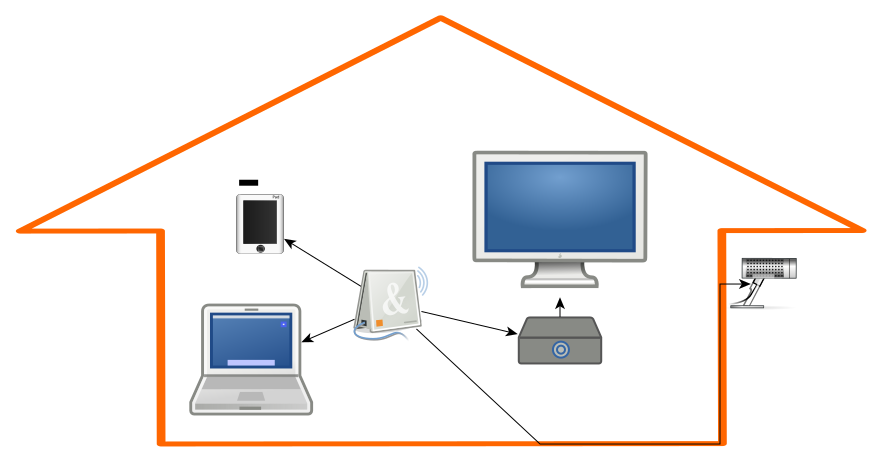
\includegraphics[width=0.7\textwidth]{intro-digitalhome}
\caption{Exemple de réseau domestique}
\end{figure}

Le réseau domestique est formé par l'ensemble des appareils se trouvent dans une maison. Ce réseau est déjà capable de fournir des services tels que le partage de contenus entre un disque dur en réseau (ou \textit{NAS}) sur la télévision ou sur les ordinateurs. L'étape suivante du développement de cette approche est l'introduction de capteurs et d'actuateurs (domotique).

Les opérateurs télécoms qui fournissent des équipements et des services sont bien souvent en difficultés pour dépanner les utilisateurs. Une des raisons de ce problème est notamment le manque d'informations sur le système. Le service après-vente ne possède pas de moyen de connaître la topologie du réseau (utilisation de \textit{wifi} ou courant porteur), la configuration de certains équipements et encore moins l'état de fonctionnement des équipements, des liens réseau ou des services.

Ce cadre applicatif a fourni les cas d'études et d'expérimentation à cette thèse. Ils réunissent les caractéristiques que nous avons introduites en~\ref{sec:intro:problematique}.
\begin{itemize}
	\item Le réseau domestique est composé de dispositifs hétérogènes.
	\item Chaque équipement fournit ses propres données sous des schémas que nous ne maîtrisons pas.
	\item Les paramètres de configuration et d'autres données accessibles via des services spécifiques sont des données persistantes. Il est possible de récupérer des données de métriques pour mesurer la santé du réseau.
	\item Des requêtes hybrides sont nécessaire pour former des alarmes basées sur des données persistantes (catalogue, agrégats historiques).
	\item Plusieurs types d'utilisateurs avec des métiers différents observent ce réseau.
\end{itemize}

Les travaux développés dans cette thèse contribuent à un système d'observation applicable sur tout système. Nous validerons notre approche par son application sur la compréhension du réseau local domestique. Ceci pourra être utilisé pour aider les diagnostics faits au service après-vente.
